\scanpage{58}
\[
u_r:\widetilde{\mathcal G}_3\xrightarrow{\sim}\widetilde{\mathcal G}_J
\]
et tout repère $r'$ \inserted{\unsure{au $=$ $\varepsilon$ près|avec $=$ $\varepsilon$ pour $r$}} sera de la forme de façon unique
\[
r'=rg_0\quad\text{avec }g_0\in\widetilde{\mathcal G}_3
\]
\[
(38)\quad\text{i.e.}\quad u_{r'}=u_ru_{g_0}\qquad(\text{avec }u_r(g_0)=g\text{ mais peu importe})
\]
d'où, en passant à l'action sur les $\Pi_1$ en $P_+$ resp. $P_\varepsilon$, on trouve
\[
(39)\qquad \psi_{r'\deleted{\unsure{\varepsilon}}}=\psi_r\circ\Pi_1(g_0,P_+)\qquad\text{si }r'=r\circ g_0.
\]
\margin{$\psi_r,\psi_{r'}$ désignent ici les isom\unsure{s}. d'épin\unsure{g}lage associés \deleted{aux} à $P_\varepsilon$.}
On va expliciter ceci pour
\[
g_0=\rho\quad\text{donc }r'=r\rho=(\omega i,\omega,\unsure{\bar\omega|\varpi})\quad\text{si }r=(i,\omega,\unsure{\bar\omega|\varpi})
\]
On trouve
\[
\psi_\varepsilon^{\omega i,\omega}=\inserted{\rho_\omega\circ\psi_\varepsilon^{i,\omega}=}\psi_\varepsilon^{i,\omega}\circ\rho
\]
où on a identifié $\rho$ aussi à un élément de $\widetilde\Pi_{0,3}$, et à l'autom qu'il induit sur $\Pi_{0,3}$.

\uline{NB} $\rho_\omega$ est la rotation autour de $P_\varepsilon,P_{\varepsilon'}$ d'un tiers de tour, \deleted{\unsure{suivant}} l'orientation $\omega$ sur l'équateur.

\margin{\uline{NB}\quad $\psi_\varepsilon^{i,\omega}(l_0),\psi_\varepsilon^{i,\omega}(l_1),\deleted{\unsure{\psi_\varepsilon^{i,\omega}(l_0)}}$ sont resp. les lacets \unsure{tournant|fondés} à partir de $P_\varepsilon$, autour des trous $R_{\omega i},R_{\unsure{\omega^2}i}$, \deleted{\unsure{qui}} passant $Q_i$ (donc \unsure{au détriment de} $\unsure{R_i|R_{\omega\prime i}}$ : \unsure{$R_{\omega i}\cdots$}), et dans le sens d'orientation $\unsure{\bar\omega|\varpi}=\omega\wedge\varepsilon$.}
\figure{
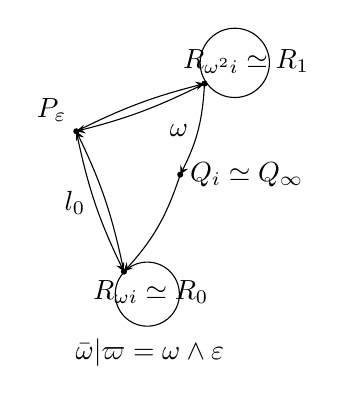
\begin{tikzpicture}[scale=1.1,>=stealth]
\coordinate (p) at (0,1);\coordinate (q) at (1.2,0.5);\coordinate (r0) at (.55,-.62);\coordinate (r1) at (1.48,1.55);
\fill (p) circle(1pt) node[above left]{$P_\varepsilon$};
\fill (q) circle(1pt) node[right]{$Q_i\simeq Q_\infty$};
\fill (r0) circle(1pt);\fill (r1) circle(1pt);
\draw (0.82,-0.88) circle (0.37);\draw (1.83,1.79) circle(0.4);
\node at(0.86,-0.86){$R_{\omega i}\simeq R_0$};\node at(1.96,1.81){$R_{\omega^2i}\simeq R_1$};
\draw[->] (p) to[bend right=7] node[left]{$l_0$} (r0);
\draw[->] (r0) to[bend right=7] (p);
\draw[->] (p) to[bend left=6] (r1);\draw[->] (r1) to[bend left=6] (p);
\draw[<-] (r0) to[bend right=12] (q);\draw[<-] (q) to[bend right=12] node[left]{$\omega$} (r1);
\node[below]at(0.85,-1.28){$\unsure{\bar\omega|\varpi}=\omega\wedge\varepsilon$};
\end{tikzpicture}}
On trouve de $=$, pour un autom qui renverse l'orientation de $\sigma$, i.e. pour un
\[
\widetilde\sigma_\infty:\quad\begin{array}{rcl}0&\longrightarrow&1\\1&\longrightarrow&0\\\infty&\longrightarrow&\infty\end{array}\qquad\deleted{\unsure{la}}\unsure{\bar\omega|\varpi}\longmapsto\unsure{\bar\omega|\varpi}'
\]
\deleted{$\unsure{\widetilde\sigma_\infty}$}
\[
g_0=\widetilde\sigma_\infty\qquad r'=r\widetilde\sigma_\infty=(\deleted{\unsure{\omega}}i,\omega',\unsure{\bar\omega|\varpi}').
\]
d'où
\[
(41)\qquad\psi_\varepsilon^{\deleted{\unsure{\omega}}i,\omega'}=\inserted{\widetilde\sigma_i\circ\psi_\varepsilon^{i,\omega}=}\psi_\varepsilon^{i,\omega}\circ\widetilde\sigma_\infty
\]
($\widetilde\sigma_i$ est la symétrie p.r. \unsure{au|du} grand cercle méridien passant par $Q_i$)
\margin{57}
